\chapter*{Présentation générale du programme d'études}
\addstarredchapter{Présentation générale du programme d'études}

\minitoc

{\AlegreyaSansLight \textit{Le présent programme est élaboré suivant l'approche par les compétences avec entrée par les situations de vie. Il s'agit, d'aller au-delà de l'acquisition des savoirs mathématiques pour rendre les élèves capables d'en faire des outils de résolution des problèmes issus des situations sus-évoquées}.}

\vspace{.5cm}

Cette orientation tient compte des évolutions en didactique, donne du sens aux apprentissages mathématiques, favorise un meilleur épanouissement intellectuel et une bonne insertion dans la société qui est la finalité principale de l'éducation au Cameroun (\textit{loi d'orientation, article 4, 1998}). Les objectifs généraux étant entre autres :

\begin{itemize}
\item de former des citoyens enracinés dans leur culture et ouverts au monde;
\item de développer la créativité, le sens de l'initiative... ;
\item d'installer la culture de l'amour de l'effort et du travail bien fait, de la quête de l'excellence... ;
\item de s'adapter aux réalités économiques ainsi qu'à l'environnement international, particulièrement en ce qui concerne la promotion des sciences et de la technologie...

A ce titre, l'enseignement des mathématiques revêt une double mission:

\begin{itemize}
\item La première est une mission de formation intellectuelle des élèves, en développant progressivement les capacités d'expérimentation, de raisonnement, de créativité et d'analyse critique, afin de les rendre capables, dans les situations de vie, d'exercer pleinement leur citoyenneté.
\item La deuxième est une mission utilitaire d'intégration des connaissances scientifiques au contexte socio économique et à l'environnement international.
\end{itemize}

Les programmes de 6ème et 5ème sont l'occasion de poser les jalons de cette double mission qui passe par le développement de trois compétences fondamentales qui sont, de manière universelle, celles de tout enseignement/apprentissage de mathématiques à savoir:

\begin{itemize}
\item Résoudre une situation problème,
\item Déployer un raisonnement mathématique,
\item Communiquer à l'aide du langage mathématique.
\end{itemize}
\end{itemize}



\section*{La situation du programme d'études dans le curriculum et sa contribution aux domaines d'apprentissage}
\addcontentsline{toc}{section}{La situation du programme d'études dans le curriculum et sa contribution aux domaines d'apprentissage}

Un \textit{curriculum} peut être perçu comme un ensemble d'actions planifiées pour susciter l'instruction (définition des objectifs, contenus, méthodes …). Un \textit{domaine d'apprentissage} pour sa part a pour fonction principale d'intégrer un ensemble de programmes d'études présentant des affinités afin de décloisonner les matières scolaires et de favoriser l'interdisciplinarité nécessaire au développement de nombreuses compétences effectives.

Le curriculum du Ministère des Enseignements Secondaires (MINESEC) a regroupé les programmes d'études dans six domaines d'apprentissage. Il s'agit des domaines suivants : langues et littérature, sciences humaines, sciences et technologies, développement personnel, arts et cultures, techniques industrielles et commerciales. Le présent programme d'études est partie intégrante du domaine d'apprentissage « Sciences et Technologies » au même titre que ceux de l'informatique et des sciences.

L'apport des mathématiques au développement de ces disciplines sœurs est incontestable. De par les nombreux outils qu'il génère (symboles, opérateurs, modèles, objets ….), ce programme offre aux disciplines sœurs, un contenu langagier et un contenu scientifique appréciables. Cela contribue à créer, à gérer et à exploiter des situations d'apprentissage qui permettent de comprendre la nature, de maîtriser des lois élémentaires et de les utiliser à bon escient.

Ce domaine est aussi celui dans lequel s'exerce par excellence le développement de la rigueur, du raisonnement, de la créativité et de la pensée critique. Les mathématiques constituent dans ce cas, un champ privilégié du développement de la pensée scientifique dans un monde en perpétuelle évolution.

\section*{Domaines de vie et contribution du programme aux domaines de vie}
\addcontentsline{toc}{section}{Domaines de vie et contribution du programme aux domaines de vie}

Les enseignements/apprentissages au MINESEC sont construits à partir de cinq domaines de vie qui sont : 
\begin{itemize}
\item la vie sociale et familiale ; 
\item la vie économique; 
\item l'environnement, le bien-être et la santé ; 
\item la citoyenneté ; 
\item les médias et communication.
\end{itemize}

Dans tous ces domaines de vie, les mathématiques jouent un rôle déterminant. Elles ont accompagné l'édification des grandes merveilles architecturales telles que les pyramides égyptiennes, balisé les trajectoires des grandes découvertes et l'exploration de l'univers aussi bien dans l'infiniment petit que dans l'infiniment grand ; elles sont à la base de l'évolution technologique du monde actuel en contribuant de manière significative à modifier notre environnement, notre mode de vie et de pensée. Elles sont enfin à la base de l'évolution de l'informatique qui a révolutionné notre manière de travailler et de communiquer.

\section*{Familles de situations couvertes par le programme d'études }
\addcontentsline{toc}{section}{Familles de situations couvertes par le programme d'études}

Une situation de vie peut être perçue comme une circonstance d'action ou de réflexion dans laquelle peut se trouver une personne. Une famille de situations renvoie à des situations de vie qui partagent au moins une propriété commune.
Dans les classes de 6ème et 5ème, quatre familles de situations ont été retenues:

\begin{enumerate}
\item Représentation, détermination des quantités et identification des objets par des nombres ;
\item Organisation des données et estimation des quantités dans la consommation des biens et services ;
\item Représentations et transformations des configurations planes dans l'environnement ;
\item Usage d'objets techniques dans la vie de tous les jours.
\end{enumerate}

Ces quatre familles permettent de passer en revue toutes les actions de la vie de tous les jours des élèves de ces niveaux :\textit{ transactions commerciales, jeux, planification des dépenses, consommation courante}, pour ne citer que celles – là. Elles sont de ce fait, les lieux de développement des compétences visées. Un module y est consacré par famille de situation et par niveau.

\section*{Modules du programme d'études}
\addcontentsline{toc}{section}{Modules du programme d'études}
\subsection*{Tableau synoptique des modules du programme d'études}
\addcontentsline{toc}{subsection}{Tableau synoptique des modules du programme d'études}

Le cours de mathématiques des classes de 6ème et 5ème est obligatoire, avec une charge horaire annuelle de 100 heures par niveau ainsi répartie :

\textbf{Premier cycle, niveau 6ème}\\

\includegraphics[width=\textwidth]{m1.pdf} 

\begin{tabular}{>{\raggedleft\arraybackslash}p{4cm}p{9cm}}
\textbf{Titre du module} & Représentation, détermination des quantités et identification des objets par des nombres.\\\midrule
\textbf{Famille de situations rattachées} & Relations et opérations fondamentales dans l'ensemble des nombres décimaux et des fractions et représentation, détermination des quantités et identification des objets par des nombres.
\end{tabular}

\includegraphics[width=\textwidth]{m2.pdf} 

\begin{tabular}{>{\raggedleft\arraybackslash}p{4cm}p{9cm}}
\textbf{Titre du module} &Organisation des données.\\\midrule
\textbf{Famille de situations rattachées} &Organisation des données et estimation des quantités dans la consommation des biens et services.
\end{tabular}

\includegraphics[width=\textwidth]{m3.pdf} 

\begin{tabular}{>{\raggedleft\arraybackslash}p{4cm}p{9cm}}
\textbf{Titre du module} & Configurations élémentaires du plan.\\\midrule
\textbf{Famille de situations rattachées} & Représentations et transformations des configurations planes dans l'environnement.
\end{tabular}

\includegraphics[width=\textwidth]{m4.pdf} 

\begin{tabular}{>{\raggedleft\arraybackslash}p{4cm}p{9cm}}
\textbf{Titre du module} & Solides de l'espace.\\\midrule
\textbf{Famille de situations rattachées} & Usage d'objets techniques dans la vie de tous les jours.
\end{tabular}

\textbf{Premier cycle, niveau 5ème}\\

\includegraphics[width=\textwidth]{m5.pdf} 

\begin{tabular}{>{\raggedleft\arraybackslash}p{4cm}p{9cm}}
\textbf{Titre du module} & Représentation, détermination des quantités et identification des objets par des nombres.\\\midrule
\textbf{Famille de situations rattachées} & Relations et opérations fondamentales dans l'ensemble des nombres décimaux et des fractions et représentation, détermination des quantités et identification des objets par des nombres.
\end{tabular}

\includegraphics[width=\textwidth]{m6.pdf} 

\begin{tabular}{>{\raggedleft\arraybackslash}p{4cm}p{9cm}}
\textbf{Titre du module} &Statistiques.\\\midrule
\textbf{Famille de situations rattachées} &Organisation des données et estimation des quantités dans la consommation des biens et services.
\end{tabular}

\includegraphics[width=\textwidth]{m7.pdf} 

\begin{tabular}{>{\raggedleft\arraybackslash}p{4cm}p{9cm}}
\textbf{Titre du module} & Configurations élémentaires du plan.\\\midrule
\textbf{Famille de situations rattachées} & Représentations et transformations des configurations planes dans l'environnement.
\end{tabular}

\includegraphics[width=\textwidth]{m8.pdf} 

\begin{tabular}{>{\raggedleft\arraybackslash}p{4cm}p{9cm}}
\textbf{Titre du module} & Solides de l'espace.\\\midrule
\textbf{Famille de situations rattachées} & Usage d'objets techniques dans la vie de tous les jours.
\end{tabular}

\subsection*{Présentation des modules}
\addcontentsline{toc}{subsection}{Présentation des modules}

Chacun des modules se présente en deux parties principales : l'\textit{introduction} et la \textit{matrice}.

L'introduction précise à l'utilisateur : la famille de situations rattachée au module, les compétences à développer, les habiletés cognitives auxquelles il fait appel.

La matrice est constituée de trois grands éléments.

\begin{center}
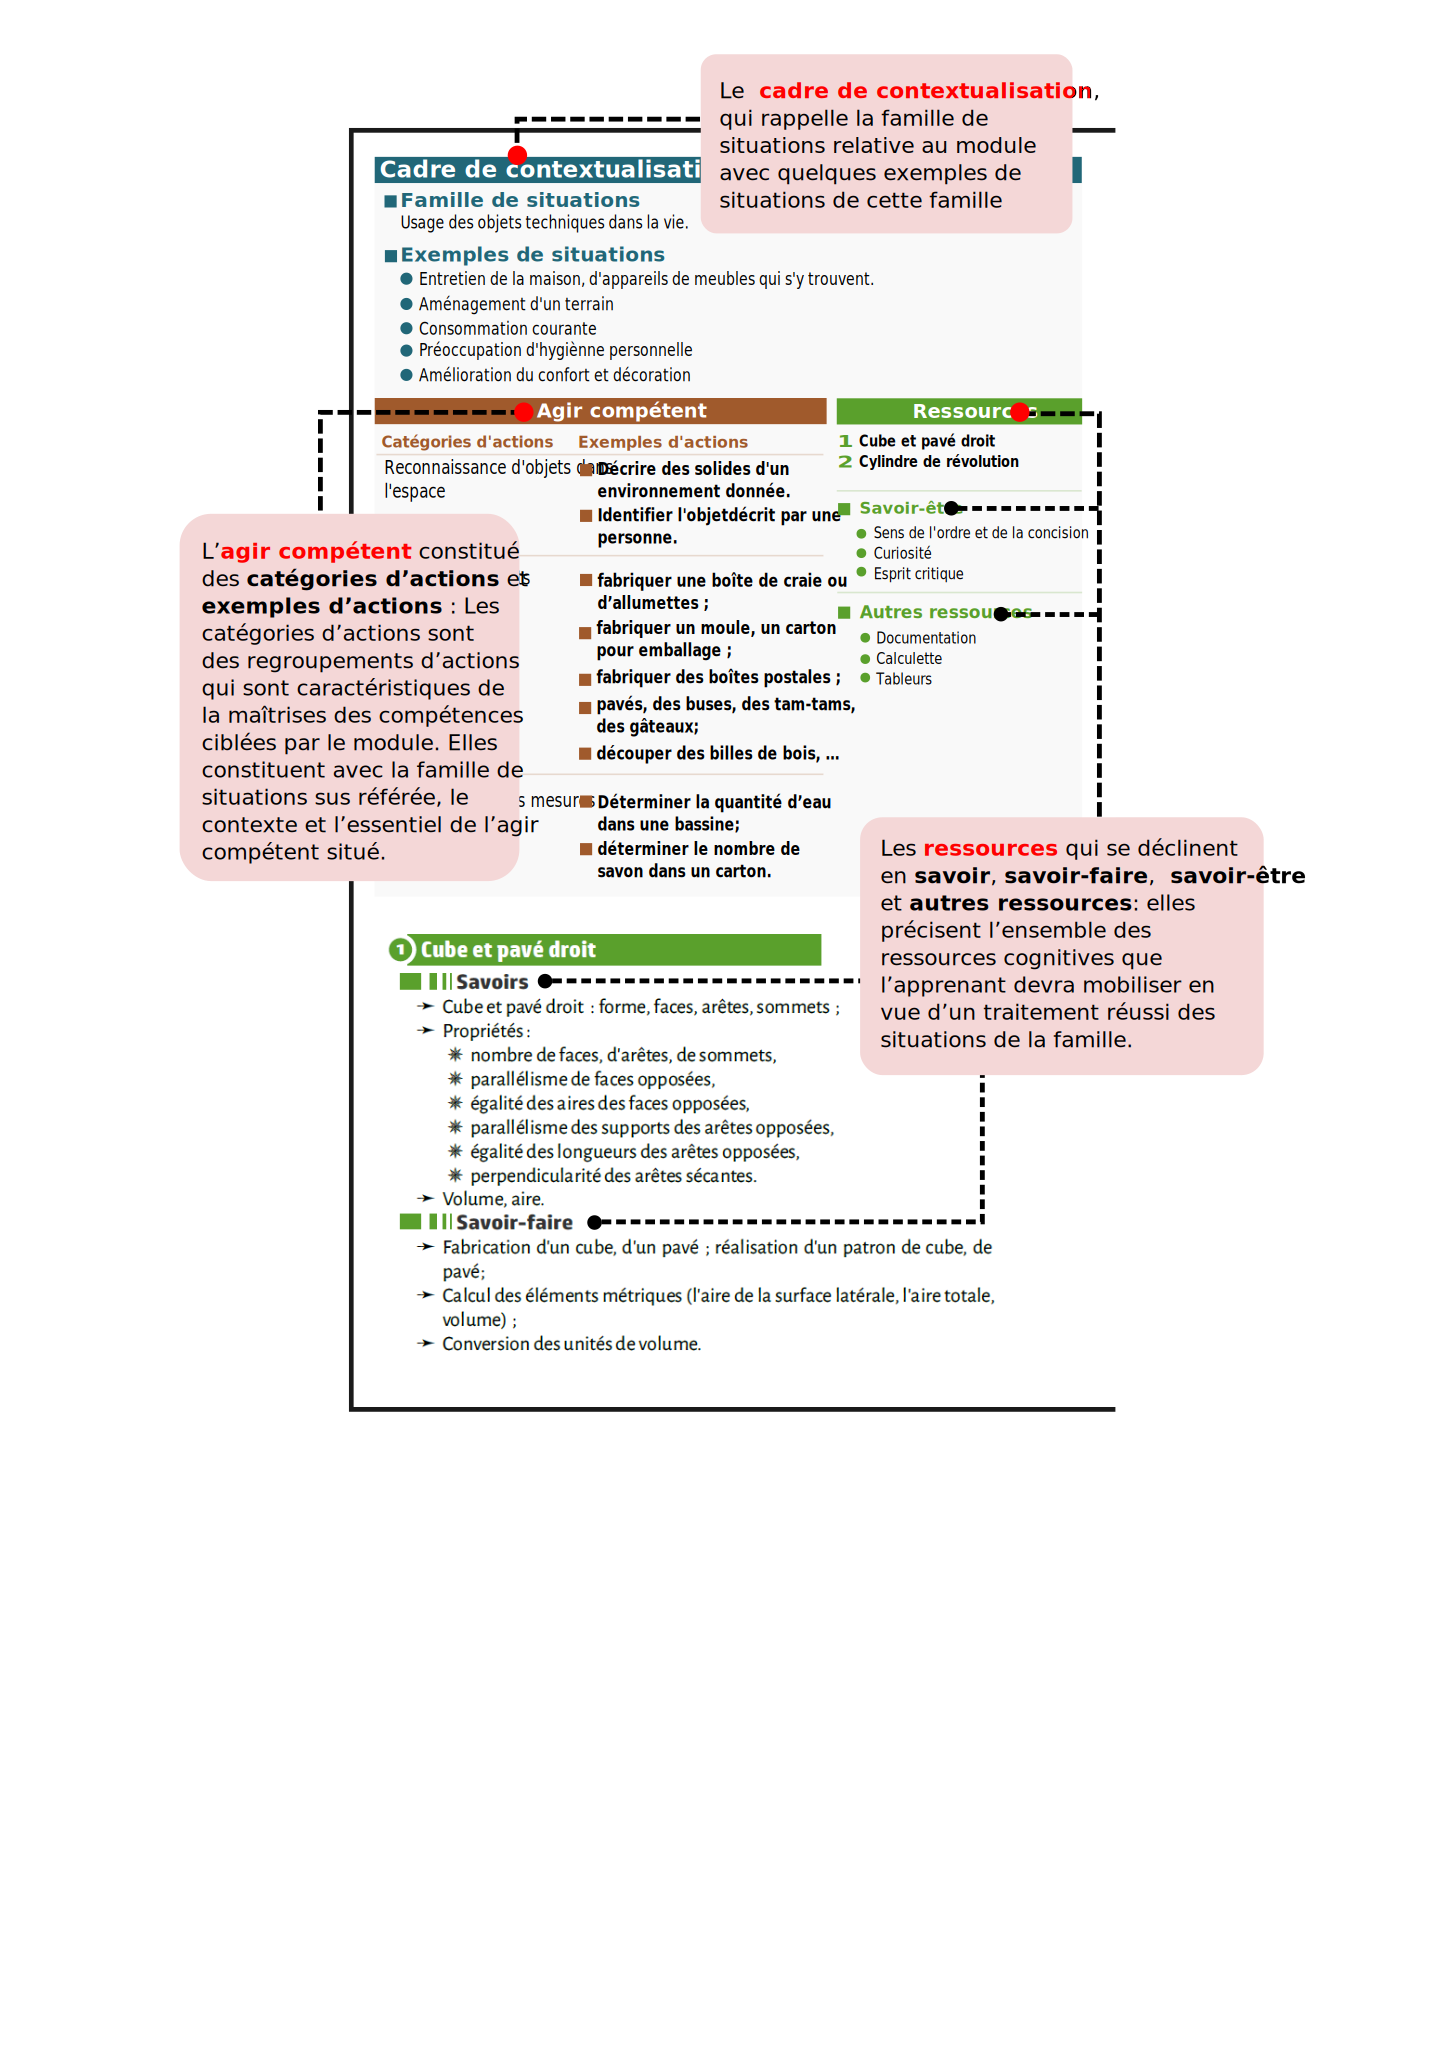
\includegraphics[width=\textwidth]{Pres.pdf}
\end{center}

\section*{Quelques recommandations d'ordre pédagogiques}
\addcontentsline{toc}{section}{Quelques recommandations d'ordre pédagogiques}
\subsection*{Méthodologie recommandée}
\addcontentsline{toc}{subsection}{Méthodologie recommandée}

L'approche par les compétences se fonde sur une pédagogie socio constructiviste. L'appropriation des savoirs mathématiques et le développement des compétences ne se transmettent pas, ils se construisent. Il importe pour cela, d'opter résolument pour une approche privilégiant l'activité de l'élève.\\
Dans cette perspective, les leçons de mathématiques doivent être basées sur des activités d'apprentissage et leur conduite doit être centrée sur l'apprenant. Aussi, chaque séquence d'enseignement/ apprentissage peut s'articuler autour des points suivants :
\begin{itemize}
\item Une introduction destinée à captiver l'attention des élèves et à contrôler les prérequis nécessaires ;
\item Une ou deux activités d'apprentissage destinées à favoriser l'acquisition des savoirs nouveaux ou à consolider des acquis antérieurs par les élèves eux-mêmes ;
\item L'essentiel à retenir en termes de notions ou de méthodes ;
\item Des exercices d'application ;
\item Des activités d'intégration si possible tant il est vrai qu'elles ont pour fonction d'amener les élèves à s'exercer sur la mobilisation de plusieurs acquis pour résoudre des problèmes courants. Elles peuvent se situer au terme de plusieurs apprentissages qui forment un tout significatif.
\item Il importe de préciser que les séances d'exercices sont des moments d'apprentissage à part entière. Elles doivent aussi être conduites de façon active.
\item Il importe aussi de comprendre que l'efficacité des actions entreprises pour rendre les élèves compétents ne s'accommode pas de la navigation à vue. L'élaboration des projets pédagogiques est de ce point de vue, une nécessité.
\end{itemize}

\subsection*{Evaluation}
\addcontentsline{toc}{subsection}{Evaluation}

Chaque épreuve écrite de contrôle des apprentissages devra tenir compte de l'évaluation des savoirs mathématiques et de l'évaluation des compétences, le tout encastré dans une charpente ayant les deux parties suivantes :
\begin{enumerate}
\item  \textbf{Travaux numériques }: Il s'agit par exemple d'évaluer la capacité à pratiquer le calcul exact, approché ou littéral ; à gérer des situations de vie par lecture/construction des tableaux ou par identification/résolution des modèles mathématiques sous-jacents ….
\item \textbf{Travaux géométriques} : Ils peuvent évaluer la capacité à représenter des objets usuels du plan, à décrire ou à caractériser des solides de l'espace, à calculer des grandeurs rattachées à ces objets, à gérer des situations de vie par l'utilisation de ces objets, …
\end{enumerate}
Les évaluations orales pendant les séances de classe sont encouragées. Elles permettent d'évaluer chez les élèves la capacité à communiquer en langage mathématique qui est l'une des compétences fondamentales de cette discipline ; elles constituent aussi, une source de motivation pour les élèves.\\
Les niveaux d'exigence ne doivent pas excéder le troisième niveau de la\textit{ taxonomie de BLOOM}. Ils doivent alors se limiter à la connaissance, la compréhension ou l'application (relativement simple).

\subsection*{Quelques consignes relatives aux contenus et aux apprentissages}
\addcontentsline{toc}{subsection}{Quelques consignes relatives aux contenus et aux apprentissages}
\subsubsection*{Langage ensembliste}
\addcontentsline{toc}{subsubsection}{Langage ensembliste}
Le professeur introduira, progressivement et à chaque fois que cela sera nécessaire, les notions et symboles ensemblistes $\emptyset, \in, \notin, \subset, \cup$ et $\cap$.\\
Il ne saurait être question de traiter la théorie des ensembles pour elle-même. De même, on introduira les notations des ensembles de nombres :  $\G N, \G Z$ et $\G D$ sans pour autant faire de leçon spécifique sur chaque ensemble.
\subsubsection*{Comparaison des nombres}
\addcontentsline{toc}{subsubsection}{Comparaison des nombres}
On habituera, tout au long du cycle, les élèves à utiliser un support graphique pour visualiser des notions numériques (comparaison, encadrement).
\subsubsection*{Calculatrices}
\addcontentsline{toc}{subsubsection}{Calculatrices}
La calculatrice est un outil qui, avec ou sans instructions officielles, connaît une large diffusion. Il est de l'intérêt des enseignants d'en tenir compte. S'il ne peut
être question, vu les coûts, d'imposer son usage par des mentions dans les programmes officiels, il importe de recenser à tous les niveaux les points de programmes et les
activités motivant son emploi et favorisant chez l'élève l'habitude d'une utilisation intelligente.
\subsubsection*{Apprentissage de la rigueur et abus de langage}
\addcontentsline{toc}{subsubsection}{Apprentissage de la rigueur et abus de langage}
Le professeur conduira progressivement les élèves au niveau de rigueur de langage souhaitable, mais tolérera les abus consistant à confondre par exemple
longueur et mesure. On ne se privera pas d'utiliser des formulations habituelles telles que :"\textit{La longueur du segment est 5 cm}" ou "\textit{un segment de 5 cm}", "\textit{Une surface de 3 cm$²$} ", "L\textit{e volume du prisme est de 4 l} ","\textit{Un angle de 30$^{\circ}$} ".
\subsubsection*{Angles}
\addcontentsline{toc}{subsubsection}{Angle}
Les notions d'angle et de secteur angulaire sont des notions difficiles à mettre en place de façon rigoureuse. Préférence sera donnée à être en accord avec le langage courant.
\subsubsection*{Espace}
\addcontentsline{toc}{subsubsection}{Espace}
L'étude de l'espace est répartie sur la totalité du cursus. Le problème de la représentation plane de configurations de l'espace se pose ; cette représentation ne
peut pas suppléer l'observation effective et, si possible, la construction des solides sera effectuée par les élèves.
\subsubsection*{Configurations planes}
\addcontentsline{toc}{subsubsection}{Configurations planes}
On s'efforcera de présenter des configurations planes que l'élève peut rencontrer hors de l'école ou qu'il peut réemployer (exemples de polygones réguliers en
classe de 5ème pour pouvoir proposer ultérieurement des exemples de prisme droit à base régulière). Mais, il ne peut être question de leur donner la même place qu'aux
configurations fondamentales, outils de raisonnement couramment employés; on demandera à l'élève de justifier, par exemple, qu'un triangle est équilatéral; on se
contentera, par contre, de lui demander de reconnaître un hexagone. On n'oubliera pas de proposer aux élèves des cas de figures trop souvent délaissés (exemple :
triangle avec un angle obtus pour la recherche des hauteurs et de l'orthocentre).
\subsubsection{Gestion des modules}
\addcontentsline{toc}{subsubsection}{Gestion des modules}
Dans l'ensemble un module forme un tout cohérent, mais il ne serait pas pertinent de terminer un module avant de commencer le suivant ; nous conseillons donc
au professeur d'alterner les activités numériques et les activités géométriques : par exemple on pourra étudier de front les modules 1 et 3, 2 et 4 pour la classe de sixième
et les modules 5 et 7, 6 et 8 pour la classe de cinquième.